HTTPのresponseパケットを見てみることにしましょう。構造は以下のとおりです:

\begin{lstlisting}[numbers=none]
HTTP/1.1 200 OK     //ステータス行
Server: nginx/1.0.8 //サーバが使用するWEBソフトウェアの名称及びバージョン
Date:Date: Tue, 30 Oct 2012 04:14:25 GMT //送信時刻
Content-Type: text/html   //サーバが送信するデータの型
Transfer-Encoding: chunked //送信するHTTPパケットが分解されることを表しています。
Connection: keep-alive   //コネクション状態の保持
Content-Length: 90        //ボディの内容の長さ
//空行 ヘッダとボディを分けるために使われます。
<!DOCTYPE html PUBLIC "-//W3C//DTD XHTML 1.0 Transitional//EN"... //ボディ
\end{lstlisting}

レスポンスパケットの第一行はステータス行と呼ばれ、HTTPプロトコルバージョン番号、ステータスコード、及びステータスメッセージの3つの部分から構成されています。

ステータスコードはHTTPクライアントにHTTPサーバが事前にResponseを発生させるか伝えます。HTTP/1.1プロトコルでは5種類のステータスコードが定義されています。ステータスコードは3桁の数字で表されます。はじめの数字はレスポンスの型を定義しています。

\begin{description}
  \item[1XX] 情報の表示 - リクエストの取得に成功しました。継続して処理します。
  \item[2XX] 成功 - リクエストの取得に成功しました。わかりました。受け付けます。
  \item[3XX] リダイレクション - リクエストを完了させる為に一歩進んだ処理が必要です。
  \item[4XX] クライアントエラー - リクエストにシンタックスエラーまたはリクエストを実現できません。
  \item[5XX] サーバーエラー - サーバは合法なリクエストを実現できません。
\end{description}

下の図で詳細なレスポンス情報について説明しております。左側にたくさんのリソースのレスポンスコードを見ることができます。200は通常です。正常なデータであることを意味しています。302ははリダイレクトを意味します。response headerの中には詳細な情報が展開されています。

\begin{figure}[H]
  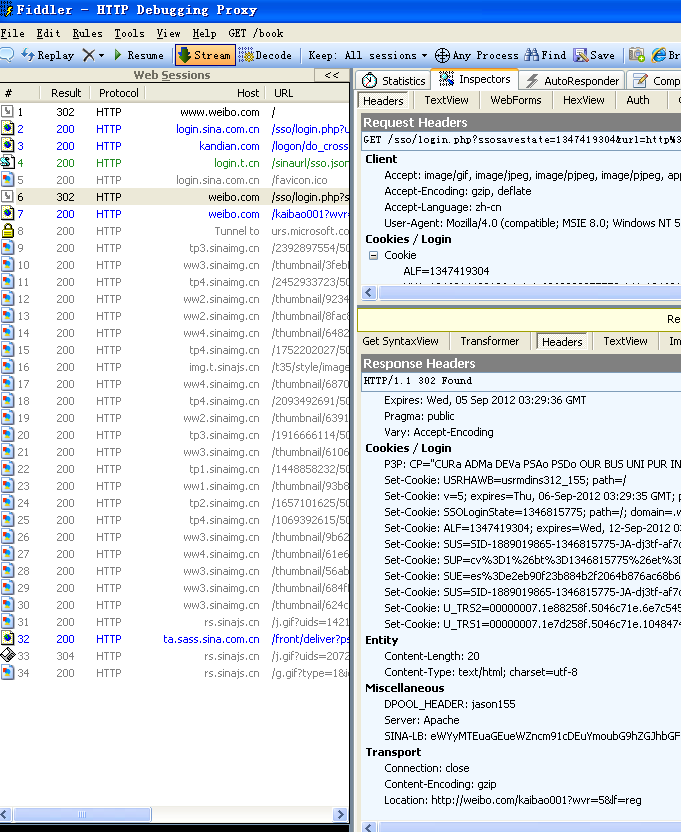
\includegraphics[width=14cm]{3.1.response.png}
   \label{図3.6}
   \caption{ホームページに一度訪問した場合のリクエスト情報のすべて}
\end{figure}


